% Lecture 11: exact content reconstruction of source slides 51--112 from
% Lecture9/Linear algebra_ 06_4.pptx. No source slide is embedded as an image.
% Compile from the repository root with:
%   pdflatex -interaction=nonstopmode -halt-on-error -output-directory=Lecture11 Lecture11/lecture11.tex
\pdfminorversion=7
\documentclass[aspectratio=169]{beamer}

\usepackage{amsmath,amssymb,mathtools}
\usepackage{array,booktabs,multirow}
\usepackage{xcolor}
\usepackage{tikz}
\usepackage{iftex}
\ifPDFTeX
  \usepackage[UTF8,heading=false]{ctex}
\else
  \usepackage{fontspec}
  \usepackage{xeCJK}
  \setCJKmainfont{Microsoft YaHei}
\fi
\usetikzlibrary{arrows.meta,calc,positioning}

\makeatletter
\def\input@path{{./}{../}{Lecture11/}}
\makeatother

\mode<presentation>{
  \usetheme{OSUCSE169}
  \setbeamercovered{invisible}
}
\setbeamertemplate{navigation symbols}{}
\setbeamertemplate{footline}[frame number]
\setbeamercolor{headline}{fg=black,bg=black}
\setbeamercolor{section in head/foot}{bg=gray}
\setbeamertemplate{headline}{%
  \begin{beamercolorbox}[ht=2.25ex,dp=3.75ex]{section in head/foot}
    \insertnavigation{\paperwidth}
  \end{beamercolorbox}}

\definecolor{lecturegreen}{RGB}{48,105,21}
\definecolor{sourcecyan}{RGB}{0,132,166}
\definecolor{sourceblue}{RGB}{0,112,192}
\definecolor{diagramblue}{RGB}{0,174,239}

\newcommand{\R}{\mathbb{R}}
\newcommand{\vect}[1]{\mathbf{#1}}
\newcommand{\Span}{\operatorname{Span}}
\newcommand{\Col}{\operatorname{Col}}
\newcommand{\Nul}{\operatorname{Nul}}
\newcommand{\Row}{\operatorname{Row}}
\newcommand{\sourcehead}[1]{\textcolor{sourcecyan}{\textbf{#1}}}
\newcommand{\coord}[2]{\left[#1\right]_{#2}}
\newcommand{\chaptercard}[4]{%
  \begin{frame}[plain]
    \vfill
    {\Huge\color{lecturegreen}\bfseries #1}\hspace{1.2em}%
    {\Huge\color{sourcecyan} #2}
    \vspace{2.4cm}

    {\Huge\color{sourcecyan}\bfseries #3}\par\medskip
    {\LARGE\color{sourcecyan}\bfseries #4}
    \vfill
  \end{frame}}

\begin{document}
% Source slide 51
\section[4.4 Coordinate Systems]{4.4 Coordinate Systems}
\chaptercard{4}{Vector Spaces}{4.4}{COORDINATE SYSTEMS}

% Source slide 52
\begin{frame}[shrink=7]{THE UNIQUE REPRESENTATION THEOREM}
\begin{itemize}
\item \sourcehead{Theorem 7:} Let $B=\{\vect b_1,\ldots,\vect b_n\}$ be a basis for vector space $V$. Then for each $\vect x$ in $V$, there exists a unique set of scalars $c_1,\ldots,c_n$ such that
\begin{equation}
\vect x=c_1\vect b_1+\cdots+c_n\vect b_n. \tag{1}
\end{equation}
\item \textbf{Proof:} Since $B$ spans $V$, there exist scalars such that (1) holds.
\item Suppose $\vect x$ also has the representation
\[
\vect x=d_1\vect b_1+\cdots+d_n\vect b_n
\]
for scalars $d_1,\ldots,d_n$.
\end{itemize}
\end{frame}

% Source slide 53
\begin{frame}[shrink=9]{THE UNIQUE REPRESENTATION THEOREM}
\begin{itemize}
\item Then, subtracting, we have
\begin{equation}
0=\vect x-\vect x=(c_1-d_1)\vect b_1+\cdots+(c_n-d_n)\vect b_n. \tag{2}
\end{equation}
\item Since $B$ is linearly independent, the weights in (2) must all be zero. That is, $c_j=d_j$ for $1\leq j\leq n$.
\item \textbf{Definition:} Suppose $B=\{\vect b_1,\ldots,\vect b_n\}$ is a basis for $V$ and $\vect x$ is in $V$. The \textbf{coordinates of $\vect x$ relative to the basis $B$} (or the \textbf{$B$-coordinate of $\vect x$}) are the weights $c_1,\ldots,c_n$ such that
\[
\vect x=c_1\vect b_1+\cdots+c_n\vect b_n.
\]
\end{itemize}
\end{frame}

% Source slide 54
\begin{frame}[shrink=7]{THE UNIQUE REPRESENTATION THEOREM}
\begin{itemize}
\item If $c_1,\ldots,c_n$ are the $B$-coordinates of $\vect x$, then the vector in $\R^n$
\[
\coord{\vect x}{B}=\begin{bmatrix}c_1\\ \vdots\\ c_n\end{bmatrix}
\]
is the \textbf{coordinate vector of $\vect x$ (relative to $B$)}, or the \textbf{$B$-coordinatevector of$\vect x$}.
\item The mapping $\vect x\mapsto\coord{\vect x}{B}$ is the \textbf{coordinate mapping (determined by $B$)}.
\end{itemize}
\end{frame}

% Source slide 55
\begin{frame}[shrink=12]{COORDINATES IN $\R^n$}
\begin{itemize}
\item When a basis $B$ for $\R^n$ is fixed, the $B$-coordinate vector of a specified $\vect x$ is easily found, as in the example below.
\item \textbf{Example 1:} Let
\[
\vect b_1=\begin{bmatrix}2\\1\end{bmatrix},\qquad
\vect b_2=\begin{bmatrix}-1\\1\end{bmatrix},\qquad
\vect x=\begin{bmatrix}4\\5\end{bmatrix},
\]
and $B=\{\vect b_1,\vect b_2\}$. Find the coordinate vector $\coord{\vect x}{B}$ of $\vect x$ relative to $B$.
\item \textbf{Solution:} The $B$-coordinate $c_1,c_2$ of $\vect x$ satisfy
\[
c_1\underbrace{\begin{bmatrix}2\\1\end{bmatrix}}_{\vect b_1}
+c_2\underbrace{\begin{bmatrix}-1\\1\end{bmatrix}}_{\vect b_2}
=\underbrace{\begin{bmatrix}4\\5\end{bmatrix}}_{\vect x}.
\]
\end{itemize}
\end{frame}

% Source slide 56
\begin{frame}[shrink=8]{COORDINATES IN $\R^n$}
or
\begin{equation}
\underbrace{\begin{bmatrix}2&-1\\1&1\end{bmatrix}}_{\vect b_1\quad\vect b_2}
\begin{bmatrix}c_1\\c_2\end{bmatrix}
=\underbrace{\begin{bmatrix}4\\5\end{bmatrix}}_{\vect x}. \tag{3}
\end{equation}
\begin{itemize}
\item This equation can be solved by row operations on an augmented matrix or by using the inverse of the matrix on the left.
\item In any case, the solution is $c_1=3$, $c_2=2$.
\item Thus $\vect x=3\vect b_1+2\vect b_2$ and
\[
\coord{\vect x}{B}=\begin{bmatrix}c_1\\c_2\end{bmatrix}
=\begin{bmatrix}3\\2\end{bmatrix}.
\]
\end{itemize}
\end{frame}

% Source slide 57
\begin{frame}[shrink=8]{COORDINATES IN $\R^n$}
\begin{itemize}
\item See the following figure.
\end{itemize}
\begin{columns}[T,onlytextwidth]
\begin{column}{0.48\textwidth}
\centering
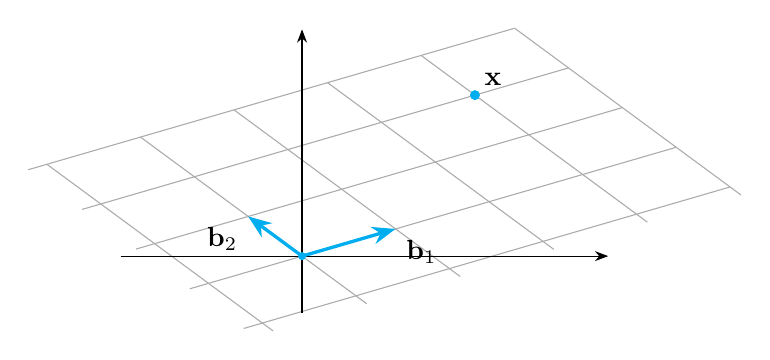
\begin{tikzpicture}[scale=.72,>=Stealth]
  \coordinate (O) at (0,0);
  \coordinate (b1) at (1.65,.48);
  \coordinate (b2) at (-.95,.70);
  \foreach \i in {-1,...,4}{
    \draw[gray!65] ($(O)+\i*(b1)-1.2*(b2)$) -- ($(O)+\i*(b1)+3.0*(b2)$);
  }
  \foreach \j in {-1,...,3}{
    \draw[gray!65] ($(O)-1.2*(b1)+\j*(b2)$) -- ($(O)+4.0*(b1)+\j*(b2)$);
  }
  \draw[->] (-3.2,0)--(5.4,0);
  \draw[->] (0,-1.0)--(0,4.0);
  \draw[diagramblue,very thick,->] (O)--(b1) node[below right,black]{$\vect b_1$};
  \draw[diagramblue,very thick,->] (O)--(b2) node[below left,black]{$\vect b_2$};
  \coordinate (x) at ($(O)+3*(b1)+2*(b2)$);
  \fill[diagramblue] (x) circle (2.5pt) node[above right,black]{$\vect x$};
  \fill[diagramblue] (O) circle (2pt);
\end{tikzpicture}

\small The $B$-coordinate vector of $\vect x$\\is $(3,2)$.
\end{column}
\begin{column}{0.50\textwidth}
\begin{itemize}
\item The matrix in (3) changes the $B$-coordinates of a vector $\vect x$ into the standard coordinates for $\vect x$.
\item An analogous change of coordinates can be carried out in $\R^n$ for a basis $B=\{\vect b_1,\ldots,\vect b_n\}$.
\item Let
\[
P_B=\begin{bmatrix}\vect b_1&\vect b_2&\cdots&\vect b_n\end{bmatrix}.
\]
\end{itemize}
\end{column}
\end{columns}
\end{frame}

% Source slide 58
\begin{frame}[shrink=8]{COORDINATES IN $\R^n$}
\begin{itemize}
\item Then the vector equation
\[
\vect x=c_1\vect b_1+c_2\vect b_2+\cdots+c_n\vect b_n
\]
is equivalent to
\begin{equation}
\vect x=P_B\coord{\vect x}{B}. \tag{4}
\end{equation}
\item $P_B$ is called the \textbf{change-of-coordinates matrix from $B$ to the standard basis in $\R^n$}.
\item Left-multiplication by $P_B$ transforms the coordinate vector $\coord{\vect x}{B}$ into $\vect x$.
\item Since the columns of $P_B$ form a basis for $\R^n$, $P_B$ is invertible (by the Invertible Matrix Theorem).
\end{itemize}
\end{frame}

% Source slide 59
\begin{frame}[shrink=7]{COORDINATES IN $\R^n$}
\begin{itemize}
\item Left-multiplication by $P_B^{-1}$ converts $\vect x$ into its $B$-coordinate vector:
\[
P_B^{-1}\vect x=\coord{\vect x}{B}.
\]
\item The correspondence $\vect x\mapsto\coord{\vect x}{B}$, produced by $P_B^{-1}$, is the coordinate mapping.
\item Since $P_B^{-1}$ is an invertible matrix, the coordinate mapping is a one-to-one linear transformation from $\R^n$ onto $\R^n$, by the Invertible Matrix Theorem.
\end{itemize}
\end{frame}

% Source slide 60
\begin{frame}[shrink=8]{THE COORDINATE MAPPING}
\begin{itemize}
\item \sourcehead{Theorem 8:} Let $B=\{\vect b_1,\ldots,\vect b_n\}$ be a basis for a vector space $V$. Then the coordinate mapping $\vect x\mapsto\coord{\vect x}{B}$ is a one-to-one linear transformation from $V$ onto $\R^n$.
\item \textbf{Proof:} Take two typical vectors in $V$, say,
\[
\vect u=c_1\vect b_1+\cdots+c_n\vect b_n,
\qquad
\vect w=d_1\vect b_1+\cdots+d_n\vect b_n.
\]
\item Then, using vector operations,
\[
\vect u+\vect v=(c_1+d_1)\vect b_1+\cdots+(c_n+d_n)\vect b_n.
\]
\end{itemize}
\end{frame}

% Source slide 61
\begin{frame}[shrink=8]{THE COORDINATE MAPPING}
\begin{itemize}
\item It follows that
\[
\coord{\vect u+\vect w}{B}
=\begin{bmatrix}c_1+d_1\\\vdots\\c_n+d_n\end{bmatrix}
=\begin{bmatrix}c_1\\\vdots\\c_n\end{bmatrix}
+\begin{bmatrix}d_1\\\vdots\\d_n\end{bmatrix}
=\coord{\vect u}{B}+\coord{\vect w}{B}.
\]
\item So the coordinate mapping preserves addition.
\item If $r$ is any scalar, then
\[
r\vect u=r(c_1\vect b_1+\cdots+c_n\vect b_n)
=(rc_1)\vect b_1+\cdots+(rc_n)\vect b_n.
\]
\end{itemize}
\end{frame}

% Source slide 62
\begin{frame}[shrink=10]{THE COORDINATE MAPPING}
\begin{itemize}
\item So
\[
\coord{r\vect u}{B}=\begin{bmatrix}rc_1\\\vdots\\rc_n\end{bmatrix}
=r\begin{bmatrix}c_1\\\vdots\\c_n\end{bmatrix}
=r\coord{\vect u}{B}.
\]
\item Thus the coordinate mapping also preserves scalar multiplication and hence is a linear transformation.
\item The linearity of the coordinate mapping extends to linear combinations.
\item If $\vect u_1,\ldots,\vect u_p$ are in $V$ and if $c_1,\ldots,c_p$ are scalars, then
\begin{equation}
\coord{c_1\vect u_1+\cdots+c_p\vect u_p}{B}
=c_1\coord{\vect u_1}{B}+\cdots+c_p\coord{\vect u_p}{B}. \tag{5}
\end{equation}
\end{itemize}
\end{frame}

% Source slide 63
\begin{frame}[shrink=8]{THE COORDINATE MAPPING}
\begin{itemize}
\item In words, (5) says that the $B$-coordinate vector of a linear combination of $\vect u_1,\ldots,\vect u_p$ is the \emph{same} linear combination of their coordinate vectors.
\item The coordinate mapping in Theorem 8 is an important example of an \emph{isomorphism} from $V$ onto $\R^n$.
\item In general, a one-to-one linear transformation from a vector space $V$ onto a vector space $W$ is called an \textbf{isomorphism} from $V$ onto $W$.
\item The notation and terminology for $V$ and $W$ may differ, but the two spaces are indistinguishable as vector spaces.
\end{itemize}
\end{frame}

% Source slide 64
\begin{frame}[shrink=11]{THE COORDINATE MAPPING}
\begin{itemize}
\item \emph{Every vector space calculation in $V$ is accurately reproduced in $W$, and vice versa.}
\item In particular, any real vector space with a basis of $n$ vectors is indistinguishable from $\R^n$.
\item \textbf{Example 7:} Let
\[
\vect v_1=\begin{bmatrix}3\\6\\2\end{bmatrix},\qquad
\vect v_2=\begin{bmatrix}-1\\0\\1\end{bmatrix},\qquad
\vect x=\begin{bmatrix}3\\12\\7\end{bmatrix},
\]
and $B=\{\vect v_1,\vect v_2\}$. Then $B$ is a basis for $H=\Span\{\vect v_1,\vect v_2\}$. Determine if $\vect x$ is in $H$, and if it is, find the coordinate vector of $\vect x$ relative to $B$.
\end{itemize}
\end{frame}

% Source slide 65
\begin{frame}{THE COORDINATE MAPPING}
\begin{itemize}
\item \textbf{Solution:} If $\vect x$ is in $H$, then the following vector equation is consistent:
\[
c_1\begin{bmatrix}3\\6\\2\end{bmatrix}
+c_2\begin{bmatrix}-1\\0\\1\end{bmatrix}
=\begin{bmatrix}3\\12\\7\end{bmatrix}.
\]
\item The scalars $c_1$ and $c_2$, if they exist, are the $B$-coordinates of $\vect x$.
\end{itemize}
\end{frame}

% Source slide 66
\begin{frame}{THE COORDINATE MAPPING}
\begin{itemize}
\item Using row operations, we obtain
\[
\begin{bmatrix}3&-1&3\\6&0&12\\2&1&7\end{bmatrix}
\sim
\begin{bmatrix}1&0&2\\0&1&3\\0&0&0\end{bmatrix}.
\]
\item Thus $c_1=2$, $c_2=3$ and
\[
\coord{\vect x}{B}=\begin{bmatrix}2\\3\end{bmatrix}.
\]
\end{itemize}
\end{frame}

% Source slide 67
\begin{frame}{THE COORDINATE MAPPING}
\begin{itemize}
\item The coordinate system on $H$ determined by $B$ is shown in the following figure.
\end{itemize}
\centering
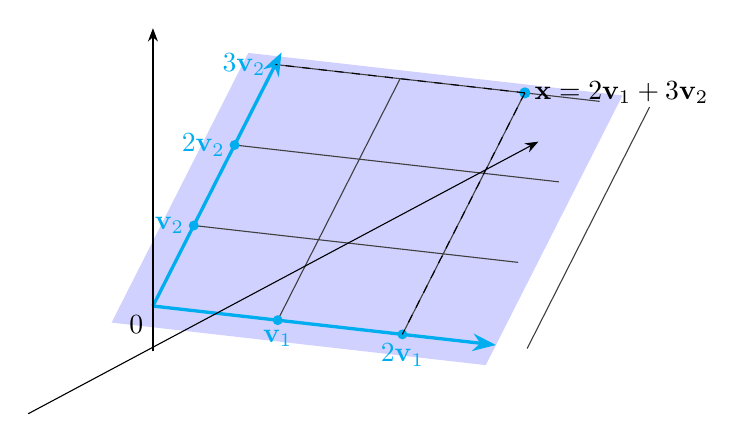
\begin{tikzpicture}[scale=.72,>=Stealth]
  \coordinate (O) at (0,0);
  \coordinate (v1) at (2.2,-.25);
  \coordinate (v2) at (.72,1.42);
  \fill[blue!18] ($(O)-.25*(v1)-.25*(v2)$) -- ($(O)+2.75*(v1)-.25*(v2)$) -- ($(O)+2.75*(v1)+3.1*(v2)$) -- ($(O)-.25*(v1)+3.1*(v2)$) -- cycle;
  \foreach \i in {0,...,3}{\draw[black!75] ($(O)+\i*(v1)$)--($(O)+\i*(v1)+3*(v2)$);}
  \foreach \j in {0,...,3}{\draw[black!75] ($(O)+\j*(v2)$)--($(O)+2.6*(v1)+\j*(v2)$);}
  \draw[diagramblue,very thick,->] (O)--($(O)+2.75*(v1)$);
  \draw[diagramblue,very thick,->] (O)--($(O)+3.15*(v2)$);
  \draw[->] (-2.2,-1.9)--(6.8,2.9);
  \draw[->] (0,-.8)--(0,4.9);
  \fill[diagramblue] (v1) circle (2.5pt) node[below]{$\vect v_1$};
  \fill[diagramblue] ($(O)+2*(v1)$) circle (2.5pt) node[below]{$2\vect v_1$};
  \fill[diagramblue] (v2) circle (2.5pt) node[left]{$\vect v_2$};
  \fill[diagramblue] ($(O)+2*(v2)$) circle (2.5pt) node[left]{$2\vect v_2$};
  \fill[diagramblue] ($(O)+3*(v2)$) circle (2.5pt) node[left]{$3\vect v_2$};
  \coordinate (x) at ($(O)+2*(v1)+3*(v2)$);
  \fill[diagramblue] (x) circle (2.8pt) node[right,black]{$\vect x=2\vect v_1+3\vect v_2$};
  \draw[dashed] (x)--($(O)+2*(v1)$);
  \draw[dashed] (x)--($(O)+3*(v2)$);
  \node[below left] at (O) {$0$};
\end{tikzpicture}

\small A coordinate system on a plane $H$ in $\R^3$.
\end{frame}

% Source slide 68
\section[4.5 Dimension]{4.5 The Dimension of a Vector Space}
\chaptercard{4}{Vector Spaces}{4.5}{THE DIMENSION OF A\\VECTOR SPACE}

% Source slide 69
\begin{frame}[shrink=8]{DIMENSION OF A VECTOR SPACE}
\begin{itemize}
\item \sourcehead{Theorem 9:} If a vector space $V$ has a basis $B=\{\vect b_1,\ldots,\vect b_n\}$, then any set in $V$ containing more than $n$ vectors must be linearly dependent.
\item \textbf{Proof:} Let $\{\vect u_1,\ldots,\vect u_p\}$ be a set in $V$ with more than $n$ vectors.
\item The coordinate vectors $\coord{\vect u_1}{B},\ldots,\coord{\vect u_p}{B}$ form a linearly dependent set in $\R^n$, because there are more vectors ($p$) than entries ($n$) in each vector.
\end{itemize}
\end{frame}

% Source slide 70
\begin{frame}[shrink=8]{DIMENSION OF A VECTOR SPACE}
\begin{itemize}
\item So there exist scalars $c_1,\ldots,c_p$, not all zero, such that
\[
c_1\coord{\vect u_1}{B}+\cdots+c_p\coord{\vect u_p}{B}
=\underbrace{\begin{bmatrix}0\\\vdots\\0\end{bmatrix}}_{\textcolor{sourceblue}{\text{The zero vector in }\R^n}}.
\]
\item Since the coordinate mapping is a linear transformation,
\[
\coord{c_1\vect u_1+\cdots+c_p\vect u_p}{B}
=\begin{bmatrix}0\\\vdots\\0\end{bmatrix}.
\]
\end{itemize}
\end{frame}

% Source slide 71
\begin{frame}[shrink=8]{DIMENSION OF A VECTOR SPACE}
\begin{itemize}
\item The zero vector on the right displays the $n$ weights needed to build the vector $c_1\vect u_1+\cdots+c_p\vect u_p$ from the basis vectors in $B$.
\item That is,
\[
c_1\vect u_1+\cdots+c_p\vect u_p=0\cdot\vect b_1+\cdots+0\cdot\vect b_n=0.
\]
\item Since the $c_i$ are not all zero, $\{\vect u_1,\ldots,\vect u_p\}$ is linearly dependent.
\item Theorem 9 implies that if a vector space $V$ has a basis $B=\{\vect b_1,\ldots,\vect b_n\}$, then each linearly independent set in $V$ has no more than $n$ vectors.
\end{itemize}
\end{frame}

% Source slide 72
\begin{frame}[shrink=7]{DIMENSION OF A VECTOR SPACE}
\begin{itemize}
\item \sourcehead{Theorem 10:} If a vector space $V$ has a basis of $n$ vectors, then every basis of $V$ must consist of exactly $n$ vectors.
\item \textbf{Proof:} Let $B_1$ be a basis of $n$ vectors and $B_2$ be any other basis (of $V$).
\item Since $B_1$ is a basis and $B_2$ is linearly independent, $B_2$ has no more than $n$ vectors, by Theorem 9.
\item Also, since $B_2$ is a basis and $B_1$ is linearly independent, $B_2$ has at least $n$ vectors.
\item Thus $B_2$ consists of exactly $n$ vectors.
\end{itemize}
\end{frame}

% Source slide 73
\begin{frame}[shrink=12]{DIMENSION OF A VECTOR SPACE}
\begin{itemize}
\item \textbf{Definition:} If $V$ is spanned by a finite set, then $V$ is said to be \textbf{finite-dimensional}, and the \textbf{dimension} of $V$, written as $\dim V$, is the number of vectors in a basis for $V$. The dimension of the zero vector space $\{0\}$ is defined to be zero. If $V$ is not spanned by a finite set, then $V$ is said to be \textbf{infinite-dimensional}.
\item \textbf{Example 3:} Find the dimension of the subspace
\[
H=\left\{\begin{bmatrix}
a-3b+6c\\
5a+4d\\
b-2c-d\\
5d
\end{bmatrix}:a,b,c,d\text{ in }\R\right\}.
\]
\end{itemize}
\end{frame}

% Source slide 74
\begin{frame}[shrink=10]{DIMENSION OF A VECTOR SPACE}
\begin{itemize}
\item $H$ is the set of all linear combinations of the vectors
\[
\vect v_1=\begin{bmatrix}1\\5\\0\\0\end{bmatrix},\quad
\vect v_2=\begin{bmatrix}-3\\0\\1\\0\end{bmatrix},\quad
\vect v_3=\begin{bmatrix}6\\0\\-2\\0\end{bmatrix},\quad
\vect v_4=\begin{bmatrix}0\\4\\-1\\5\end{bmatrix}.
\]
\item Clearly, $\vect v_1\neq0$, $\vect v_2$ is not a multiple of $\vect v_1$, but $\vect v_3$ is a multiple of $\vect v_2$.
\item By the Spanning Set Theorem, we may discard $\vect v_3$ and still have a set that spans $H$.
\end{itemize}
\end{frame}

% Source slide 75
\begin{frame}[shrink=8]{SUBSPACES OF A FINITE-DIMENSIONAL SPACE}
\begin{itemize}
\item Finally, $\vect v_4$ is not a linear combination of $\vect v_1$ and $\vect v_2$.
\item So $\{\vect v_1,\vect v_2,\vect v_4\}$ is linearly independent and hence is a basis for $H$.
\item Thus $\dim H=3$.
\item \sourcehead{Theorem 11:} Let $H$ be a subspace of a finite-dimensional vector space $V$. Any linearly independent set in $H$ can be expanded, if necessary, to a basis for $H$. Also, $H$ is finite-dimensional and
\[
\dim H\leq\dim V.
\]
\end{itemize}
\end{frame}

% Source slide 76
\begin{frame}[shrink=7]{SUBSPACES OF A FINITE-DIMENSIONAL SPACE}
\begin{itemize}
\item \textbf{Proof:} If $H=\{0\}$, then certainly $\dim H=0\leq\dim V$.
\item Otherwise, let $S=\{\vect u_1,\ldots,\vect u_k\}$ be any linearly independent set in $H$.
\item If $S$ spans $H$, then $S$ is a basis for $H$.
\item Otherwise, there is some $\vect u_{k+1}$ in $H$ that is not in $\Span S$.
\end{itemize}
\vfill
{\tiny \copyright\ 2016 Pearson Education, Ltd.}
\end{frame}

% Source slide 77
\begin{frame}[shrink=8]{SUBSPACES OF A FINITE-DIMENSIONAL SPACE}
\begin{itemize}
\item But then $\{\vect u_1,\ldots,\vect u_k,\vect u_{k+1}\}$ will be linearly independent, because no vector in the set can be a linear combination of vectors that precede it (by Theorem 4).
\item So long as the new set does not span $H$, we can continue this process of expanding $S$ to a larger linearly independent set in $H$.
\item But the number of vectors in a linearly independent expansion of $S$ can never exceed the dimension of $V$, by Theorem 9.
\end{itemize}
\end{frame}

% Source slide 78
\begin{frame}[shrink=9]{THE BASIS THEOREM}
\begin{itemize}
\item So eventually the expansion of $S$ will span $H$ and hence will be a basis for $H$, and $\dim H\leq\dim V$.
\item \sourcehead{Theorem 12:} Let $V$ be a $p$-dimensional vector space, $p\geq1$. Any linearly independent set of exactly $p$ elements in $V$ is automatically a basis for $V$. Any set of exactly $p$ elements that spans $V$ is automatically a basis for $V$.
\item \textbf{Proof:} By Theorem 11, a linearly independent set $S$ of $p$ elements can be extended to a basis for $V$.
\end{itemize}
\end{frame}

% Source slide 79
\begin{frame}{THE BASIS THEOREM}
\begin{itemize}
\item But that basis must contain exactly $p$ elements, since $\dim V=p$.
\item So $S$ must already be a basis for $V$.
\item Now suppose that $S$ has $p$ elements and spans $V$.
\item Since $V$ is nonzero, the Spanning Set Theorem implies that a subset $S'$ of $S$ is a basis of $V$.
\item Since $\dim V=p$, $S'$ must contain $p$ vectors.
\item Hence $S=S'$.
\end{itemize}
\end{frame}

% Source slide 80
\begin{frame}[shrink=7]{THE DIMENSIONS OF NUL $A$ AND COL $A$}
\begin{itemize}
\item Let $A$ be an $m\times n$ matrix, and suppose the equation $A\vect x=0$ has $k$ free variables.
\item A spanning set for $\Nul A$ will produce exactly $k$ linearly independent vectors---say, $\vect u_1,\ldots,\vect u_k$---one for each free variable.
\item So $\{\vect u_1,\ldots,\vect u_k\}$ is a basis for $\Nul A$, and the number of free variables determines the size of the basis.
\end{itemize}
\end{frame}

% Source slide 81
\begin{frame}[shrink=8]{DIMENSIONS OF NUL $A$ AND COL $A$}
\begin{itemize}
\item Thus, the dimension of $\Nul A$ is the number of free variables in the equation $A\vect x=0$, and the dimension of $\Col A$ is the number of pivot columns in $A$.
\item \textbf{Example 5:} Find the dimensions of the null space and the column space of
\[
A=\begin{bmatrix}
-3&6&-1&1&-7\\
1&-2&2&3&-1\\
2&-4&5&8&-4
\end{bmatrix}.
\]
\end{itemize}
\end{frame}

% Source slide 82
\begin{frame}[shrink=8]{DIMENSIONS OF NUL $A$ AND COL $A$}
\begin{itemize}
\item \textbf{Solution:} Row reduce the augmented matrix $[A\ \ 0]$ to echelon form:
\[
\begin{bmatrix}
1&-2&2&3&-1&0\\
0&0&1&2&-2&0\\
0&0&0&0&0&0
\end{bmatrix}.
\]
\item There are three free variable---$x_2$, $x_4$ and $x_5$.
\item Hence the dimension of $\Nul A$ is 3.
\item Also $\dim\Col A=2$ because $A$ has two pivot columns.
\end{itemize}
\end{frame}

% Source slide 83
\section[4.6 Rank]{4.6 Rank}
\chaptercard{4}{Vector Spaces}{4.6}{RANK}

% Source slide 84
\begin{frame}[shrink=8]{THE ROW SPACE}
\begin{itemize}
\item If $A$ is an $m\times n$ matrix, each row of $A$ has $n$ entries and thus can be identified with a vector in $\R^n$.
\item The set of all linear combinations of the row vectors is called the \textbf{row space} of $A$ and is denoted by $\Row A$.
\item Each row has $n$ entries, so $\Row A$ is a subspace of $\R^n$.
\item Since the rows of $A$ are identified with the columns of $A^T$, we could also write $\Col A^T$ in place of $\Row A$.
\end{itemize}
\end{frame}

% Source slide 85
\begin{frame}[shrink=8]{THE ROW SPACE}
\begin{itemize}
\item \sourcehead{Theorem 13:} If two matrices $A$ and $B$ are row equivalent, then their row spaces are the same. If $B$ is in echelon form, the nonzero rows of $B$ form a basis for the row space of $A$ as well as for that of $B$.
\item \textbf{Proof:} If $B$ is obtained from $A$ by row operations, the rows of $B$ are linear combinations of the rows of $A$.
\item It follows that any linear combination of the rows of $B$ is automatically a linear combination of the rows of $A$.
\end{itemize}
\end{frame}

% Source slide 86
\begin{frame}{THE ROW SPACE}
\begin{itemize}
\item Thus the row space of $B$ is contained in the row space of $A$.
\item Since row operations are reversible, the same argument shows that the row space of $A$ is a subset of the row space of $B$.
\item So the two row spaces are the same.
\end{itemize}
\end{frame}

% Source slide 87
\begin{frame}[shrink=7]{THE ROW SPACE}
\begin{itemize}
\item If $B$ is in echelon form, its nonzero rows are linearly independent because no nonzero row is a linear combination of the nonzero rows below it. (Apply Theorem 4 to the nonzero rows of $B$ in reverse order, with the first row last).
\item Thus the nonzero rows of $B$ form a basis of the (common) row space of $B$ and $A$.
\end{itemize}
\end{frame}

% Source slide 88
\begin{frame}[shrink=9]{THE ROW SPACE}
\begin{itemize}
\item \textbf{Example 2:} Find bases for the row space, the column space, and the null space of the matrix
\[
A=\begin{bmatrix}
-2&-5&8&0&-17\\
1&3&-5&1&5\\
3&11&-19&7&1\\
1&7&-13&5&-3
\end{bmatrix}.
\]
\item \textbf{Solution:} To find bases for the row space and the column space, row reduce $A$ to an echelon form:
\end{itemize}
\end{frame}

% Source slide 89
\begin{frame}[shrink=10]{THE ROW SPACE}
\[
A\sim B=\begin{bmatrix}
1&3&-5&1&5\\
0&1&-2&2&-7\\
0&0&0&-4&20\\
0&0&0&0&0
\end{bmatrix}.
\]
\begin{itemize}
\item By Theorem 13, the first three rows of $B$ form a basis for the row space of $A$ (as well as for the row space of $B$).
\item Thus
\[
\text{Basis for }\Row A:\{(1,3,-5,1,5),(0,1,-2,2,-7),(0,0,0,-4,20)\}.
\]
\end{itemize}
\end{frame}

% Source slide 90
\begin{frame}[shrink=9]{THE ROW SPACE}
\begin{itemize}
\item For the column space, observe from $B$ that the pivots are in columns 1, 2, and 4.
\item Hence columns 1, 2, and 4 of $A$ (not $B$) form a basis for $\Col A$:
\[
\text{Basis for }\Col A:
\left\{
\begin{bmatrix}-2\\1\\3\\1\end{bmatrix},
\begin{bmatrix}-5\\3\\11\\7\end{bmatrix},
\begin{bmatrix}0\\1\\7\\5\end{bmatrix}
\right\}.
\]
\item Notice that any echelon form of $A$ provides (in its nonzero rows) a basis for $\Row A$ and also identifies the pivot columns of $A$ for $\Col A$.
\end{itemize}
\end{frame}

% Source slide 91
\begin{frame}{THE ROW SPACE}
\begin{itemize}
\item However, for $\Nul A$, we need the \emph{reduced echelon form}.
\item Further row operations on $B$ yield
\[
A\sim B\sim C=\begin{bmatrix}
1&0&1&0&1\\
0&1&-2&0&3\\
0&0&0&1&-5\\
0&0&0&0&0
\end{bmatrix}.
\]
\end{itemize}
\end{frame}

% Source slide 92
\begin{frame}[shrink=8]{THE ROW SPACE}
\begin{itemize}
\item The equation $A\vect x=0$ is equivalent to $C\vect x=0$, that is,
\begin{align*}
x_1+x_3+x_5&=0,\\
x_2-2x_3+3x_5&=0,\\
x_4-5x_5&=0.
\end{align*}
\item So $x_1=-x_3-x_5$, $x_2=2x_3-3x_5$, $x_4=5x_5$, with $x_3$ and $x_5$ free variables.
\end{itemize}
\end{frame}

% Source slide 93
\begin{frame}[shrink=8]{THE ROW SPACE}
\begin{itemize}
\item The calculations show that
\[
\text{Basis for }\Nul A:
\left\{
\begin{bmatrix}-1\\2\\1\\0\\0\end{bmatrix},
\begin{bmatrix}-1\\-3\\0\\5\\1\end{bmatrix}
\right\}.
\]
\item Observe that, unlike the basis for $\Col A$, the bases for $\Row A$ and $\Nul A$ have no simple connection with the entries in $A$ itself.
\end{itemize}
\end{frame}

% Source slide 94
\begin{frame}[shrink=11]{THE RANK THEOREM}
\begin{itemize}
\item \textbf{Definition:} The \textbf{rank} of $A$ is the dimension of the column space of $A$.
\item Since $\Row A$ is the same as $\Col A^T$, the dimension of the row space of $A$ is the rank of $A^T$.
\item The dimension of the null space is sometimes called the \textbf{nullity} of $A$.
\item \sourcehead{Theorem 14:} The dimensions of the column space and the row space of an $m\times n$ matrix $A$ are equal. This common dimension, the rank of $A$, also equals the number of pivot positions in $A$ and satisfies the equation
\[
\operatorname{rank}A+\dim\Nul A=n.
\]
\end{itemize}
\end{frame}

% Source slide 95
\begin{frame}[shrink=9]{THE RANK THEOREM}
\begin{itemize}
\item \textbf{Proof:} By Theorem 6, $\operatorname{rank}A$ is the number of pivot columns in $A$.
\item Equivalently, $\operatorname{rank}A$ is the number of pivot positions in an echelon form $B$ of $A$.
\item Since $B$ has a nonzero row for each pivot, and since these rows form a basis for the row space of $A$, the rank of $A$ is also the dimension of the row space.
\item The dimension of $\Nul A$ equals the number of free variables in the equation $A\vect x=0$.
\item Expressed another way, the dimension of $\Nul A$ is the number of columns of $A$ that are \emph{not} pivot columns.
\end{itemize}
\end{frame}

% Source slide 96
\begin{frame}[shrink=8]{THE RANK THEOREM}
\begin{itemize}
\item (It is the number of these columns, not the columns themselves, that is related to $\Nul A$).
\item Obviously,
\[
\underbrace{\begin{gathered}\text{number of}\\\text{pivot columns}\end{gathered}}_{\vphantom{X}}
+
\underbrace{\begin{gathered}\text{number of}\\\text{nonpivot columns}\end{gathered}}_{\vphantom{X}}
=
\underbrace{\begin{gathered}\text{number of}\\\text{columns}\end{gathered}}_{\vphantom{X}}.
\]
\item This proves the theorem.
\end{itemize}
\end{frame}

% Source slide 97
\begin{frame}[shrink=8]{THE RANK THEOREM}
\begin{itemize}
\item \textbf{Example 3:}
\begin{itemize}
\item[a.] If $A$ is a $7\times9$ matrix with a two-dimensional null space, what is the rank of $A$?
\item[b.] Could a $6\times9$ matrix have a two-dimensional null space?
\end{itemize}
\item \textbf{Solution:}
\begin{itemize}
\item[a.] Since $A$ has 9 columns, $(\operatorname{rank}A)+2=9$, and hence $\operatorname{rank}A=7$.
\item[b.] No. If a $6\times9$ matrix, call it $B$, has a two-dimensional null space, it would have to have rank 7, by the Rank Theorem.
\end{itemize}
\end{itemize}
\end{frame}

% Source slide 98
\begin{frame}[shrink=9]{THE INVERTIBLE MATRIX THEOREM}
\textbf{(CONTINUED)}
\begin{itemize}
\item But the columns of $B$ are vectors in $\R^6$, and so the dimension of $\Col B$ cannot exceed 6; that is, $\operatorname{rank}B$ cannot exceed 6.
\item \textbf{Theorem:} Let $A$ be an $n\times n$ matrix. Then the following statements are each equivalent to the statement that $A$ is an invertible matrix.
\begin{itemize}
\item[m.] The columns of $A$ form a basis of $\R^n$.
\item[n.] $\Col A=\R^n$.
\item[o.] $\dim\Col A=n$.
\item[p.] $\operatorname{rank}A=n$.
\end{itemize}
\end{itemize}
\end{frame}

% Source slide 99
\begin{frame}[shrink=8]{RANK AND THE INVERTIBLE MATRIX THEOREM}
\begin{itemize}
\item[q.] $\Nul A=\{0\}$.
\item[r.] $\dim\Nul A=0$.
\item \textbf{Proof:} Statement (m) is logically equivalent to statements (e) and (h) regarding linear independence and spanning.
\item The other five statements are linked to the earlier ones of the theorem by the following chain of almost trivial implications:
\[
(g)\Rightarrow(n)\Rightarrow(o)\Rightarrow(p)\Rightarrow(r)\Rightarrow(q)\Rightarrow(d).
\]
\end{itemize}
\end{frame}

% Source slide 100
\begin{frame}[shrink=9]{RANK AND THE INVERTIBLE MATRIX THEOREM}
\begin{itemize}
\item Statement (g), which says that the equation $A\vect x=\vect b$ has at least one solution for each $\vect b$ in $\R^n$, implies (n), because $\Col A$ is precisely the set of all $\vect b$ such that the equation $A\vect x=\vect b$ is consistent.
\item The implications $(n)\Rightarrow(o)\Rightarrow(p)$ follow from the definitions of dimension and rank.
\item If the rank of $A$ is $n$, the number of columns of $A$, then $\dim\Nul A=0$, by the Rank Theorem, and so $\Nul A=\{0\}$.
\end{itemize}
\end{frame}

% Source slide 101
\begin{frame}{RANK AND THE INVERTIBLE MATRIX THEOREM}
\begin{itemize}
\item Thus $(p)\Rightarrow(r)\Rightarrow(q)$.
\item Also, (q) implies that the equation $A\vect x=0$ has only the trivial solution, which is statement (d).
\item Since statements (d) and (g) are already known to be equivalent to the statement that $A$ is invertible, the proof is complete.
\end{itemize}
\end{frame}

% Source slide 102
\section[4.7 Change of Basis]{4.7 Change of Basis}
\chaptercard{4}{Determinants}{4.7}{CHANGE OF BASIS}

% Source slide 103
\begin{frame}[shrink=8]{CHANGE OF BASIS}
\begin{itemize}
\item \textbf{Example 1} Consider two bases $\beta=\{\vect b_1,\vect b_2\}$ and $\mathcal C=\{\vect c_1,\vect c_2\}$ for a vector space $V$, such that
\begin{equation*}
\vect b_1=4\vect c_1+\vect c_2\quad\text{and}\quad
\vect b_2=-6\vect c_1+\vect c_2. \tag{1}
\end{equation*}
\item Suppose
\begin{equation*}
\vect x=3\vect b_1+\vect b_2. \tag{2}
\end{equation*}
\item That is, suppose $[\vect x]_{\beta}=\begin{bmatrix}3\\1\end{bmatrix}$. Find $[\vect x]_{\mathcal C}$.
\end{itemize}
\end{frame}

% Source slide 104
\begin{frame}[shrink=8]{CHANGE OF BASIS}
\begin{itemize}
\item \textbf{Solution} Apply the coordinate mapping determined by $\mathcal C$ to $\vect x$ in (2). Since the coordinate mapping is a linear transformation,
\begin{align*}
[\vect x]_{\mathcal C}&=[3\vect b_1+\vect b_2]_{\mathcal C}\\
&=3[\vect b_1]_{\mathcal C}+[\vect b_2]_{\mathcal C}.
\end{align*}
\item We can write the vector equation as a matrix equation, using the vectors in the linear combination as the columns of a matrix:
\begin{equation*}
[\vect x]_{\mathcal C}=
\begin{bmatrix}[\vect b_1]_{\mathcal C}&[\vect b_2]_{\mathcal C}\end{bmatrix}
\begin{bmatrix}3\\1\end{bmatrix}. \tag{3}
\end{equation*}
\end{itemize}
\end{frame}

% Source slide 105
\begin{frame}[shrink=8]{CHANGE OF BASIS}
\begin{itemize}
\item This formula gives $[\vect x]_{\mathcal C}$, once we know the columns of the matrix. From (1),
\[
[\vect b_1]_{\mathcal C}=\begin{bmatrix}4\\1\end{bmatrix}
\quad\text{and}\quad
[\vect b_2]_{\mathcal C}=\begin{bmatrix}-6\\1\end{bmatrix}.
\]
\item Thus, (3) provides the solution:
\[
[\vect x]_{\mathcal C}=
\begin{bmatrix}4&-6\\1&1\end{bmatrix}
\begin{bmatrix}3\\1\end{bmatrix}
=\begin{bmatrix}6\\4\end{bmatrix}.
\]
\item The $\mathcal C$-coordinates of $\vect x$ match those of the $\vect x$ in Fig. 1, as seen on the next slide.
\end{itemize}
\end{frame}

% Source slide 106
\begin{frame}{CHANGE OF BASIS}
\centering
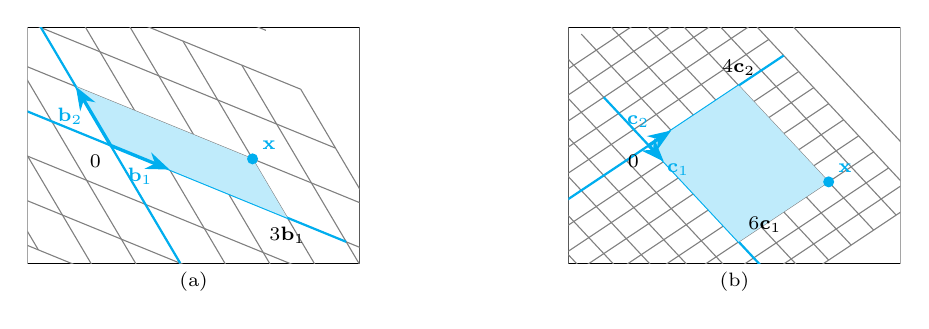
\begin{tikzpicture}[x=0.68cm,y=0.68cm,>=Stealth,font=\scriptsize]
  \begin{scope}[shift={(-7.0,0)}]
    \clip (-3.1,-2.2) rectangle (3.1,2.2);
    \draw[thin] (-3.1,-2.2) rectangle (3.1,2.2);
    \coordinate (O) at (-1.55,0);
    \coordinate (b1) at (1.10,-0.45);
    \coordinate (b2) at (-0.65,1.10);
    \foreach \i in {-3,...,5} {\draw[gray] ($(O)+\i*(b1)-3*(b2)$)--($(O)+\i*(b1)+3*(b2)$);}
    \foreach \j in {-3,...,4} {\draw[gray] ($(O)-4*(b1)+\j*(b2)$)--($(O)+5*(b1)+\j*(b2)$);}
    \draw[diagramblue,thick] ($(O)-2*(b1)$)--($(O)+4*(b1)$);
    \draw[diagramblue,thick] ($(O)-2*(b2)$)--($(O)+3*(b2)$);
    \fill[diagramblue!25] (O)--($(O)+3*(b1)$)--($(O)+3*(b1)+(b2)$)--($(O)+(b2)$)--cycle;
    \draw[->,diagramblue,very thick] (O)--($(O)+(b1)$) node[midway,below] {$\vect b_1$};
    \draw[->,diagramblue,very thick] (O)--($(O)+(b2)$) node[midway,left] {$\vect b_2$};
    \fill[diagramblue] ($(O)+3*(b1)+(b2)$) circle (2pt) node[above right] {$\vect x$};
    \node[below left] at (O) {$0$};
    \node[below] at ($(O)+3*(b1)$) {$3\vect b_1$};
  \end{scope}
  \begin{scope}[shift={(3.1,0)}]
    \clip (-3.1,-2.2) rectangle (3.1,2.2);
    \draw[thin] (-3.1,-2.2) rectangle (3.1,2.2);
    \coordinate (P) at (-1.60,0);
    \coordinate (c1) at (0.28,-0.30);
    \coordinate (c2) at (0.42,0.28);
    \foreach \i in {-5,...,9} {\draw[gray] ($(P)+\i*(c1)-5*(c2)$)--($(P)+\i*(c1)+6*(c2)$);}
    \foreach \j in {-6,...,7} {\draw[gray] ($(P)-6*(c1)+\j*(c2)$)--($(P)+9*(c1)+\j*(c2)$);}
    \draw[diagramblue,thick] ($(P)-3*(c1)$)--($(P)+8*(c1)$);
    \draw[diagramblue,thick] ($(P)-4*(c2)$)--($(P)+6*(c2)$);
    \fill[diagramblue!25] (P)--($(P)+6*(c1)$)--($(P)+6*(c1)+4*(c2)$)--($(P)+4*(c2)$)--cycle;
    \draw[->,diagramblue,very thick] (P)--($(P)+(c1)$) node[midway,below right] {$\vect c_1$};
    \draw[->,diagramblue,very thick] (P)--($(P)+(c2)$) node[midway,above left] {$\vect c_2$};
    \fill[diagramblue] ($(P)+6*(c1)+4*(c2)$) circle (2pt) node[above right] {$\vect x$};
    \node[below left] at (P) {$0$};
    \node[above right] at ($(P)+6*(c1)$) {$6\vect c_1$};
    \node[above] at ($(P)+4*(c2)$) {$4\vect c_2$};
  \end{scope}
  \node at (-7,-2.55) {(a)};
  \node at (3.1,-2.55) {(b)};
\end{tikzpicture}

\vspace{0.25em}
\begin{flushleft}
\textbf{FIGURE 1}\quad Two coordinate systems for the same vector space.
\end{flushleft}
\end{frame}

% Source slide 107
\begin{frame}[shrink=8]{CHANGE OF BASIS}
\begin{itemize}
\item \sourcehead{Theorem 15:} Let $\beta=\{\vect b_1,\ldots,\vect b_n\}$ and $\mathcal C=\{\vect c_1,\ldots,\vect c_2\}$ for a vector space $V$. Then there is a unique $n\times n$ matrix $P_{\mathcal C\leftarrow\beta}$ such that
\begin{equation*}
[\vect x]_{\mathcal C}=P_{\mathcal C\leftarrow\beta}[\vect x]_{\beta}. \tag{4}
\end{equation*}
\item The columns of $P_{\mathcal C\leftarrow\beta}$ are the $\mathcal C$-coordinate vectors of the vectors in the basis $\beta$. That is,
\begin{equation*}
P_{\mathcal C\leftarrow\beta}=
\begin{bmatrix}[\vect b_1]_{\mathcal C}&[\vect b_2]_{\mathcal C}&\cdots&[\vect b_n]_{\mathcal C}\end{bmatrix}. \tag{5}
\end{equation*}
\end{itemize}
\end{frame}

% Source slide 108
\begin{frame}[shrink=5]{CHANGE OF BASIS}
\begin{itemize}
\item The matrix $P_{\mathcal C\leftarrow\beta}$ in Theorem 15 is called the \textbf{change-of-coordinates matrix from $\beta$ to $\mathcal C$}. Multiplication by $P_{\mathcal C\leftarrow\beta}$ converts $\beta$-coordinates into $\mathcal C$-coordinates.
\item Figure 2 below illustrates the change-of-coordinates equation (4).
\end{itemize}
\centering
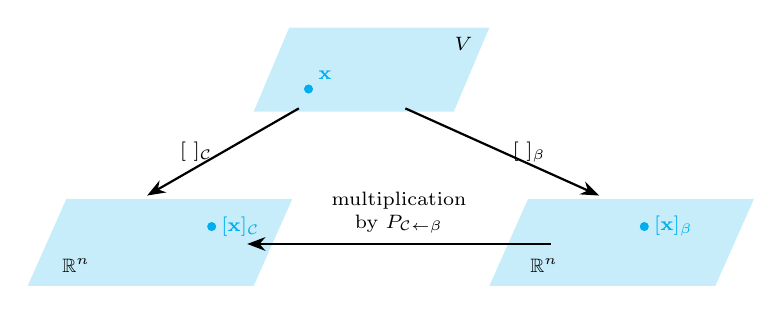
\begin{tikzpicture}[>=Stealth,font=\scriptsize,scale=.82]
  \fill[diagramblue!22] (-1.5,2.5)--(1.6,2.5)--(2.15,3.8)--(-.95,3.8)--cycle;
  \node at (1.75,3.55) {$V$};
  \fill[diagramblue] (-.65,2.85) circle (2pt) node[above right] {$\vect x$};
  \fill[diagramblue!22] (-5,-.2)--(-1.5,-.2)--(-.9,1.15)--(-4.4,1.15)--cycle;
  \fill[diagramblue!22] (2.15,-.2)--(5.65,-.2)--(6.25,1.15)--(2.75,1.15)--cycle;
  \fill[diagramblue] (-2.15,.72) circle (2pt) node[right] {$[\vect x]_{\mathcal C}$};
  \fill[diagramblue] (4.55,.72) circle (2pt) node[right] {$[\vect x]_{\beta}$};
  \node at (-4.25,.12) {$\R^n$};
  \node at (3.0,.12) {$\R^n$};
  \draw[->,thick] (-.8,2.55)--(-3.15,1.2) node[midway,left] {$[\ ]_{\mathcal C}$};
  \draw[->,thick] (.85,2.55)--(3.85,1.2) node[midway,right] {$[\ ]_{\beta}$};
  \draw[->,thick] (3.1,.45)--(-1.6,.45) node[midway,above,align=center] {multiplication\\by $P_{\mathcal C\leftarrow\beta}$};
\end{tikzpicture}

\begin{flushleft}
\textbf{FIGURE 2}\quad Two coordinate systems for $V$.
\end{flushleft}
\end{frame}

% Source slide 109
\begin{frame}[shrink=9]{CHANGE OF BASIS}
\begin{itemize}
\item The columns of $P_{\mathcal C\leftarrow\beta}$ are linearly independent because they are the coordinate vectors of the linearly independent set $\beta$.
\item Since $P_{\mathcal C\leftarrow\beta}$ is square, it must be invertible, by the Invertible Matrix Theorem. Left-multiplying both sides of equation (4) by $(P_{\mathcal C\leftarrow\beta})^{-1}$ yields
\[
(P_{\mathcal C\leftarrow\beta})^{-1}[\vect x]_{\mathcal C}=[\vect x]_{\beta}.
\]
\item Thus $(P_{\mathcal C\leftarrow\beta})^{-1}$ is the matrix that converts $\mathcal C$-coordinates into $\beta$--coordinates. That is,
\begin{equation*}
(P_{\mathcal C\leftarrow\beta})^{-1}=P_{\beta\leftarrow\mathcal C}. \tag{6}
\end{equation*}
\end{itemize}
\end{frame}

% Source slide 110
\begin{frame}[shrink=10]{CHANGE OF BASIS IN $\R^n$}
\begin{itemize}
\item If $\beta=\{\vect b_1,\ldots,\vect b_n\}$ and $\mathcal E$ is the standard basis $\{\vect e_1,\ldots,\vect e_n\}$ in $\R^n$, then $[\vect b_1]_{\mathcal E}=\vect b_1$, and likewise for the other vectors in $\beta$. In this case, $P_{\mathcal E\leftarrow\beta}$ is thesame as the change-of-coordinates matrix $P_{\beta}$ introduced in Section 4.4, namely,
\[
P_{\beta}=\begin{bmatrix}\vect b_1&\vect b_2&\cdots&\vect b_n\end{bmatrix}.
\]
\item To change coordinates between two nonstandard bases in $\R^n$,we need Theorem 15. The theorem shows that to solve the change-of-basis problem, we need the coordinate vectors of the old basis relative to the new basis.
\end{itemize}
\end{frame}

% Source slide 111
\begin{frame}[shrink=12]{CHANGE OF BASIS IN $\R^n$}
\begin{itemize}
\item \textbf{Example 2} Let
$\vect b_1=\begin{bmatrix}-9\\1\end{bmatrix}$,
$\vect b_2=\begin{bmatrix}-5\\-1\end{bmatrix}$,
$\vect c_1=\begin{bmatrix}1\\-4\end{bmatrix}$,
$\vect c_2=\begin{bmatrix}3\\-5\end{bmatrix}$
and consider the bases for $\R^n$ given by $\beta=\{\vect b_1,\vect b_2\}$ and $\mathcal C=\{\vect c_1,\vect c_2\}$. Find the change-of-coordinates matrix from $\beta$ to $\mathcal C$.
\item \textbf{Solution} The matrix $P_{\beta\leftarrow\mathcal C}$ involves the $\mathcal C$-coordinate vectors of $\vect b_1$ and $\vect b_2$. Let $[\vect b_1]_{\mathcal C}=\begin{bmatrix}x_1\\x_2\end{bmatrix}$ and $[\vect b_2]_{\mathcal C}=\begin{bmatrix}y_1\\y_2\end{bmatrix}$. Then, by definition,
\[
\begin{bmatrix}\vect c_1&\vect c_2\end{bmatrix}\begin{bmatrix}x_1\\x_2\end{bmatrix}=\vect b_1
\quad\text{and}\quad
\begin{bmatrix}\vect c_1&\vect c_2\end{bmatrix}\begin{bmatrix}y_1\\y_2\end{bmatrix}=\vect b_2.
\]
\end{itemize}
\end{frame}

% Source slide 112
\begin{frame}[shrink=10]{CHANGE OF BASIS IN $\R^n$}
\begin{itemize}
\item To solve both systems simultaneously, augment the coefficient matrix with $\vect b_1$ and $\vect b_2$, and row reduce:
\begin{equation*}
\left[\begin{array}{cc|cc}\vect c_1&\vect c_2&\vect b_1&\vect b_2\end{array}\right]=
\left[\begin{array}{cc|cc}1&3&-9&-5\\-4&-5&1&-1\end{array}\right]
\sim
\left[\begin{array}{cc|cc}1&0&6&4\\0&1&-5&-3\end{array}\right]. \tag{7}
\end{equation*}
\item Thus
\[
[\vect b_1]_{\mathcal C}=\begin{bmatrix}6\\-5\end{bmatrix}
\quad\text{and}\quad
[\vect b_2]_{\mathcal C}=\begin{bmatrix}4\\-3\end{bmatrix}.
\]
\item The desired change-of-coordinates matrix is therefore
\[
P_{\mathcal C\leftarrow\beta}=
\begin{bmatrix}[\vect b_1]_{\mathcal C}&[\vect b_2]_{\mathcal C}\end{bmatrix}
=\begin{bmatrix}6&4\\-5&-3\end{bmatrix}.
\]
\end{itemize}
\end{frame}

\end{document}
